\documentclass[table, 12pt]{article}
\usepackage[T1]{fontenc}
\usepackage[utf8]{inputenc}
\usepackage[english]{babel}
\usepackage{graphicx}
\usepackage{titlesec}
\usepackage{hyperref}
\usepackage[usenames,dvipsnames]{xcolor}
\usepackage{float}
\usepackage[export]{adjustbox}
\usepackage{longtable}
\usepackage{mathtools}
\usepackage[most]{tcolorbox}
\newcounter{testexample}
\usepackage{xparse}
\usepackage{subcaption}
\usepackage{amsmath}


\titleformat{\paragraph}
{\normalfont\normalsize\bfseries}{\theparagraph}{1em}{}
\titlespacing*{\paragraph}
{0pt}{3.25ex plus 1ex minus .2ex}{1.5ex plus .2ex}

\NewDocumentEnvironment{testexample}{ O{} }
{
\colorlet{colexam}{teal!60!black} % Global example color
\newtcolorbox[use counter=testexample]{testexamplebox}{%
    % Example Frame Start
    empty,% Empty previously set parameters
    title={\exampletext #1},% use \thetcbcounter to access the testexample counter text
    % Attaching a box requires an overlay
    attach boxed title to top left,
       % Ensures proper line breaking in longer titles
       minipage boxed title,
    % (boxed title style requires an overlay)
    boxed title style={empty,size=minimal,toprule=0pt,top=4pt,left=3mm,overlay={}},
    coltitle=colexam,fonttitle=\bfseries,
    before=\par\medskip\noindent,parbox=false,boxsep=0pt,left=3mm,right=0mm,top=2pt,breakable,pad at break=0mm,
       before upper=\csname @totalleftmargin\endcsname0pt, % Use instead of parbox=true. This ensures parskip is inherited by box.
    % Handles box when it exists on one page only
    overlay unbroken={\draw[colexam,line width=.5pt] ([xshift=-0pt]title.north west) -- ([xshift=-0pt]frame.south west); },
    % Handles multipage box: first page
    overlay first={\draw[colexam,line width=.5pt] ([xshift=-0pt]title.north west) -- ([xshift=-0pt]frame.south west); },
    % Handles multipage box: middle page
    overlay middle={\draw[colexam,line width=.5pt] ([xshift=-0pt]frame.north west) -- ([xshift=-0pt]frame.south west); },
    % Handles multipage box: last page
    overlay last={\draw[colexam,line width=.5pt] ([xshift=-0pt]frame.north west) -- ([xshift=-0pt]frame.south west); },%
    }
\begin{testexamplebox}}
{\end{testexamplebox}\endlist}



\begin{document}
\begin{titlepage}
    \centering
    {\scshape\large AY 2022/2023 \par}
    \vfill
    
\includegraphics[width=100pt]{assets/logo_polimi.jpg}\par\vspace{1cm}
    {\scshape\LARGE Politecnico di Milano \par}
    \vspace{1.5cm}
    {\huge\bfseries DD\@: Design Document \par}
    \vspace{2cm}
    {\Large {Marcello De Salvo\quad Riccardo Grossoni \par Francesco Dubini}\par}
    \vfill
    {\large Professor\par
        Elisabetta \textsc{Di Nitto}}
    \vfill
    {\large \textbf{Version 0.1}\\ \today \par}
\end{titlepage}

\hypersetup{%
    pdfborder = {0 0 0}
}

\thispagestyle{plain}
\pagenumbering{gobble}
\mbox{}
\newpage
\pagenumbering{roman}
\tableofcontents
\newpage
\pagenumbering{arabic}

\section{Introduction}

\subsection{Purpose}
%The purpose of this document is to provide a full technical description of the system described in the RASD document.
%In this design document we discuss about both hardware and software architectures in terms of interaction among the components that represent the system.
%Moreover, there are mentions about the implementation, testing and integration process.
%This document will include technical language so it is primarily addressed to programmers, but stakeholders are also invited to read it in order to understand the characteristics of the development.

The objective of this document is the realization of a full technical description of the system presented in the RASD document.
Here we will analyze both hardware and software architectures, focussing on the interaction between components that constitute the system.
Additionally, we will also delve into the implementation, testing and integration process.
This document will use technical language as it's focussed to programmers, but stakeholders are also invited to read as it can be useful to understand the characteristics of the development.

\subsection{Scope}
%The scope of this design document lays in the definition of the system behavior, in both general and critical cases, and in the design of the system architecture by describing the
%logical allocation of the components and the interaction between them.
%This document also extends in part to the implementation and testing plan, where one possible course of action is explained, user interface design of user applications and requirements traceability relating to the RASD.

The scope of this design document sets down the definition of the behavior of the system, for general and critical cases, and in the design of the system architecture by analyzing the logical designation of the components and their interactions.
As stated before, this document will also delve into the implementation, the testing plan and a possible mock-up for the user interface.

\subsection{Definitions, acronyms, abbreviations}
\subsubsection*{Definitions}
\begin{itemize}
    \item \textbf{def1}: text.
    \item \textbf{def2}: text.
\end{itemize}
\subsubsection*{Acronyms}
\begin{itemize}
    \item \textbf{RASD}: Requirement Analysis and Specification Document
    \item \textbf{DD}: Design Document
    \item \textbf{ITD}: Implementation Document
    \item \textbf{API}: Application Programming Interface
    \item \textbf{DBMS}: Database Management System
    \item \textbf{DMZ}: Demilitarized Zone
    \item \textbf{OCPP}: Open Charge Point Protocol
    \item \textbf{UML}: Unified Modeling Language
    \item \textbf{GPS}: Global Positioning System
    \item \textbf{IT}: Information Technology
    \item \textbf{GUI}: Graphic User Interface
    \item \textbf{UI}: User Interface
    \item \textbf{HTTPS}:HyperText Transfer Protocol Security
    \item \textbf{HTML}: HyperText Markup Language
    \item \textbf{CSS}: Cascade Style Sheet
    \item \textbf{JS}: JavaScript
\end{itemize}

\subsection{Revision history}
\begin{itemize}
    \item Version 0.1: setup version
    \begin{itemize}
        \item[--] text 
    \end{itemize}
\end{itemize}

\subsection{Reference documents}
\begin{itemize}
    \item Specification document: "Assignment RDD AY 2022-2023"
    \item Requirements Analysis Specification Document (RASD)
    \item UML documentation: https://www.uml-diagrams.org/
    \item Slides of the lectures
\end{itemize}
\subsection{Document structure}
\begin{itemize}
    \item \textbf{Section 1} gives a brief description of the design document, it describes the purpose and the scope of it including all the definitions, acronyms and abbreviations used. 
    \item \textbf{Section 2} delves deeply into the system architecture by providing a detailed description of the components, the interfaces and all the technical choices made for the development of the application.
    It also includes detailed sequence, component and ArchiMate diagrams that describe the system in depth.
    \item \textbf{Section 3} contains a complete description of the user interface (UI), it includes all the client-side mockups with some graphs useful to understand the correct execution flow.
    \item \textbf{Section 4} maps the goals and the requirements described in the RASD to the actual functionalities presented in this DD.
    \item \textbf{Section 5} presents a description of the implementation, testing and integration phases of the system components that are going to be carried out during the technical development of the application.
\end{itemize}

\newpage

\section{Architectural Design}

\subsection{Overview}
\begin{center}
    \begin{figure}[H]
        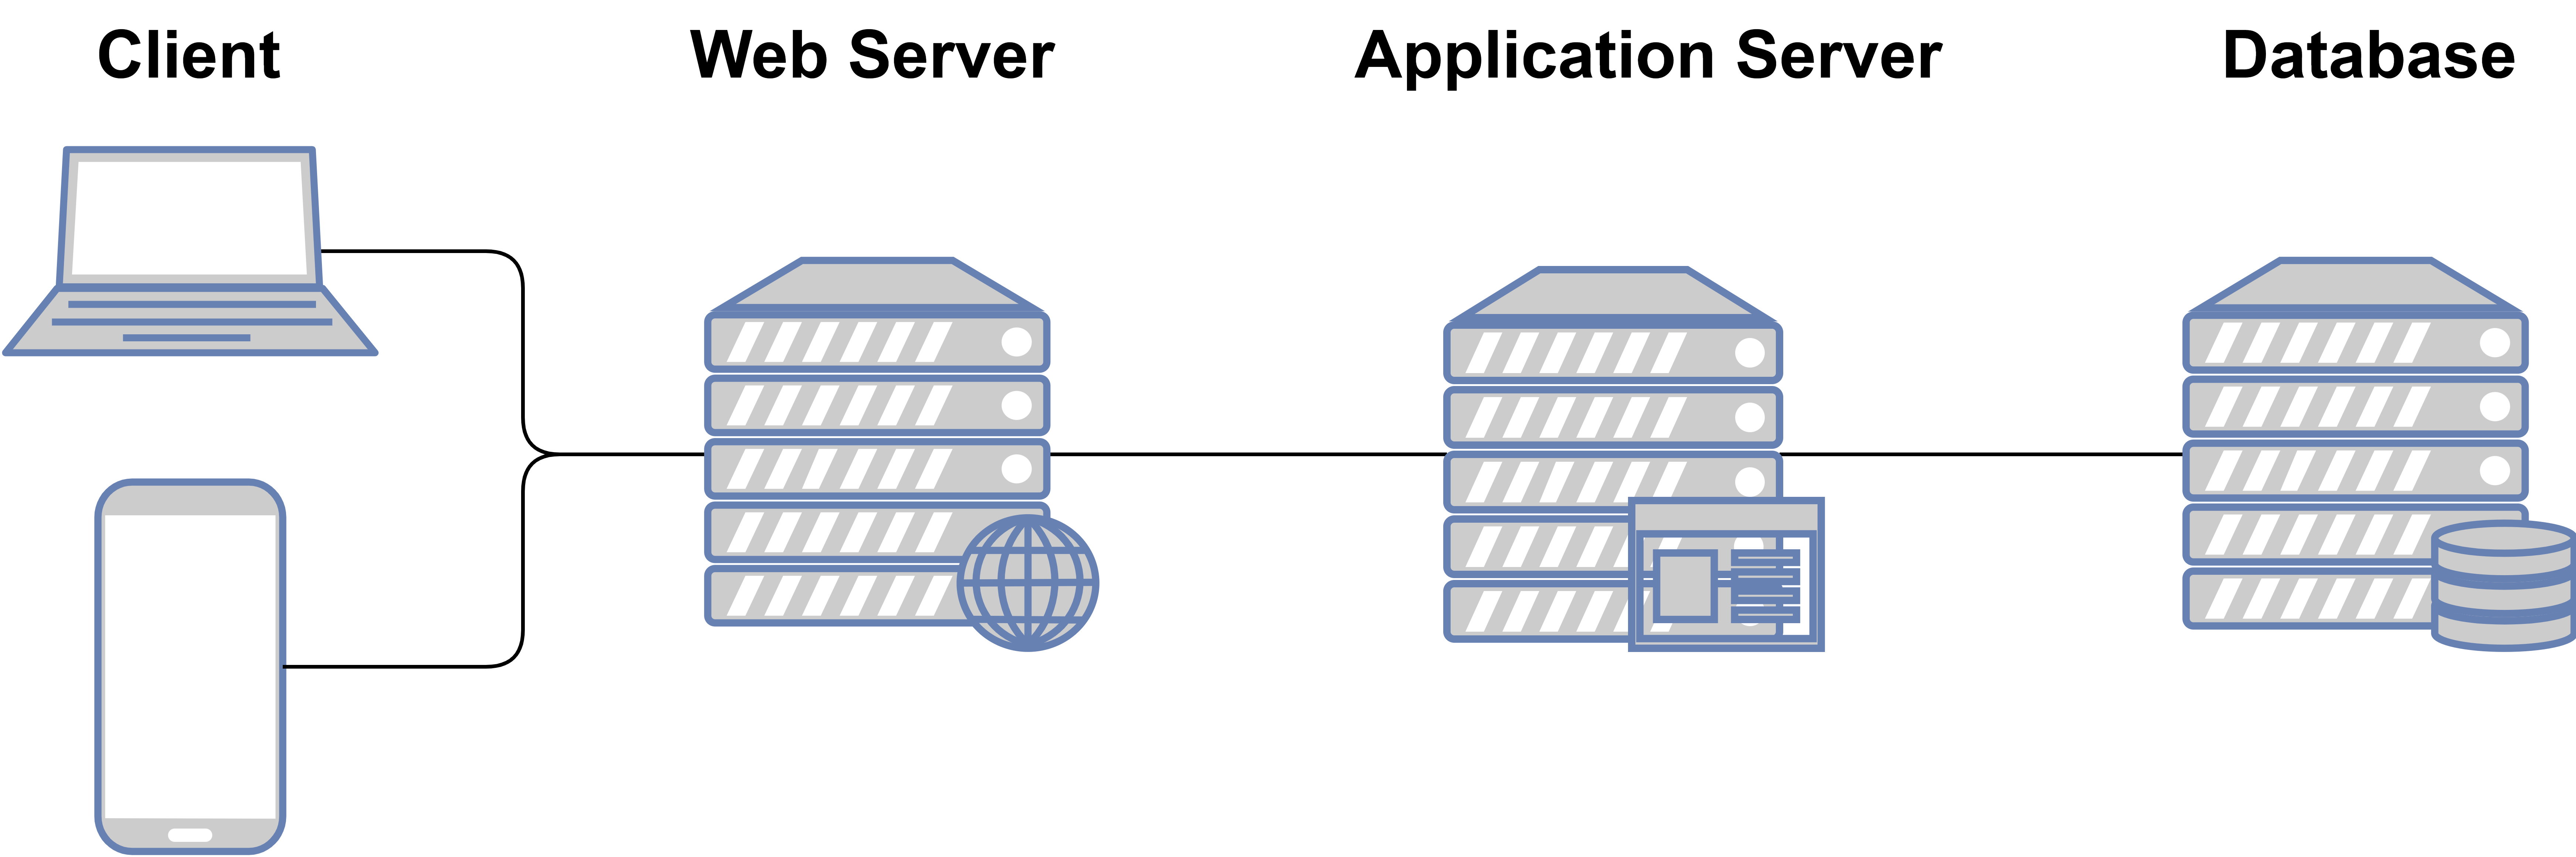
\includegraphics[scale=0.80, center]{assets/3-tier-architecture.png}
        \caption{Three Tier Architecture}
        \label{fig: three_tier_architecture}
    \end{figure}
\end{center}

The system is an application distributed across multiple devices and follows the common client-server paradigm.
The architecture is organized in three logical layers:

\begin{itemize}
    \item \textbf{Presentation Layer (P)}: It's responsible for rendering the application's user interface to the client through the Web Server. It's expressed by a GUI designed to enable the user to interact with the application efficiently.
    \item \textbf{Application Layer (A)}: It's responsible for the business logic of the application. It receives requests from the Presentation Layer, processes them, and then sends back the results to be displayed.
    \item \textbf{Data Layer(D)}: It's in charge of the access to data sources, it provides data through the database and direct it to the other layers. It's also necessary in order to grant a high level of abstraction from the database for an easy to use model.
\end{itemize}

\newpage
\begin{center}
    \begin{figure}[H]
        \includegraphics[scale=0.53, center]{assets/high_level_architecture.png}
        \caption{High Level Architecture}
        \label{fig: high_level_architecture}
    \end{figure}
\end{center}

The system's architecture, as shown in \ref{fig:high_level_architecture}, is composed by a DMZ, that includes the Web and the Mail Server in order to prevent a direct access to the internal system and improve the overall security, and firewalls that divide each newtwork segment.
To reduce computation client side a thin client is used, which allows all the heavy operations to be performed at server side. The Web Server handles the HTTP requests by the users and directs them to the Application Server, while also managing the GoogleMaps API. 
The Application Server communicates with the Database Server and elaborates data following its business logic. The Application server also handles external APIs and services, such as GoogleCalendarAPI, CarAPI, and the exetrnal CPMSs and eMSPs systems.
The Apllication Server's CPMS subsystem will also communicate with its Charging Stations and their relative sockets through the OCPP API, and with the external DSOs through their proprietary API.
The Email Server will manage all the e-mail notification by communicating with the Application Server, The database server is responsible for storing and managing the data that is used by the application. It receives requests for data from the application logic tier, retrieves the requested data from the database, and returns the data to the application logic tier.

\subsection{Component view}
\subsubsection*{General Component View}
\begin{center}
    \begin{figure}[H]
        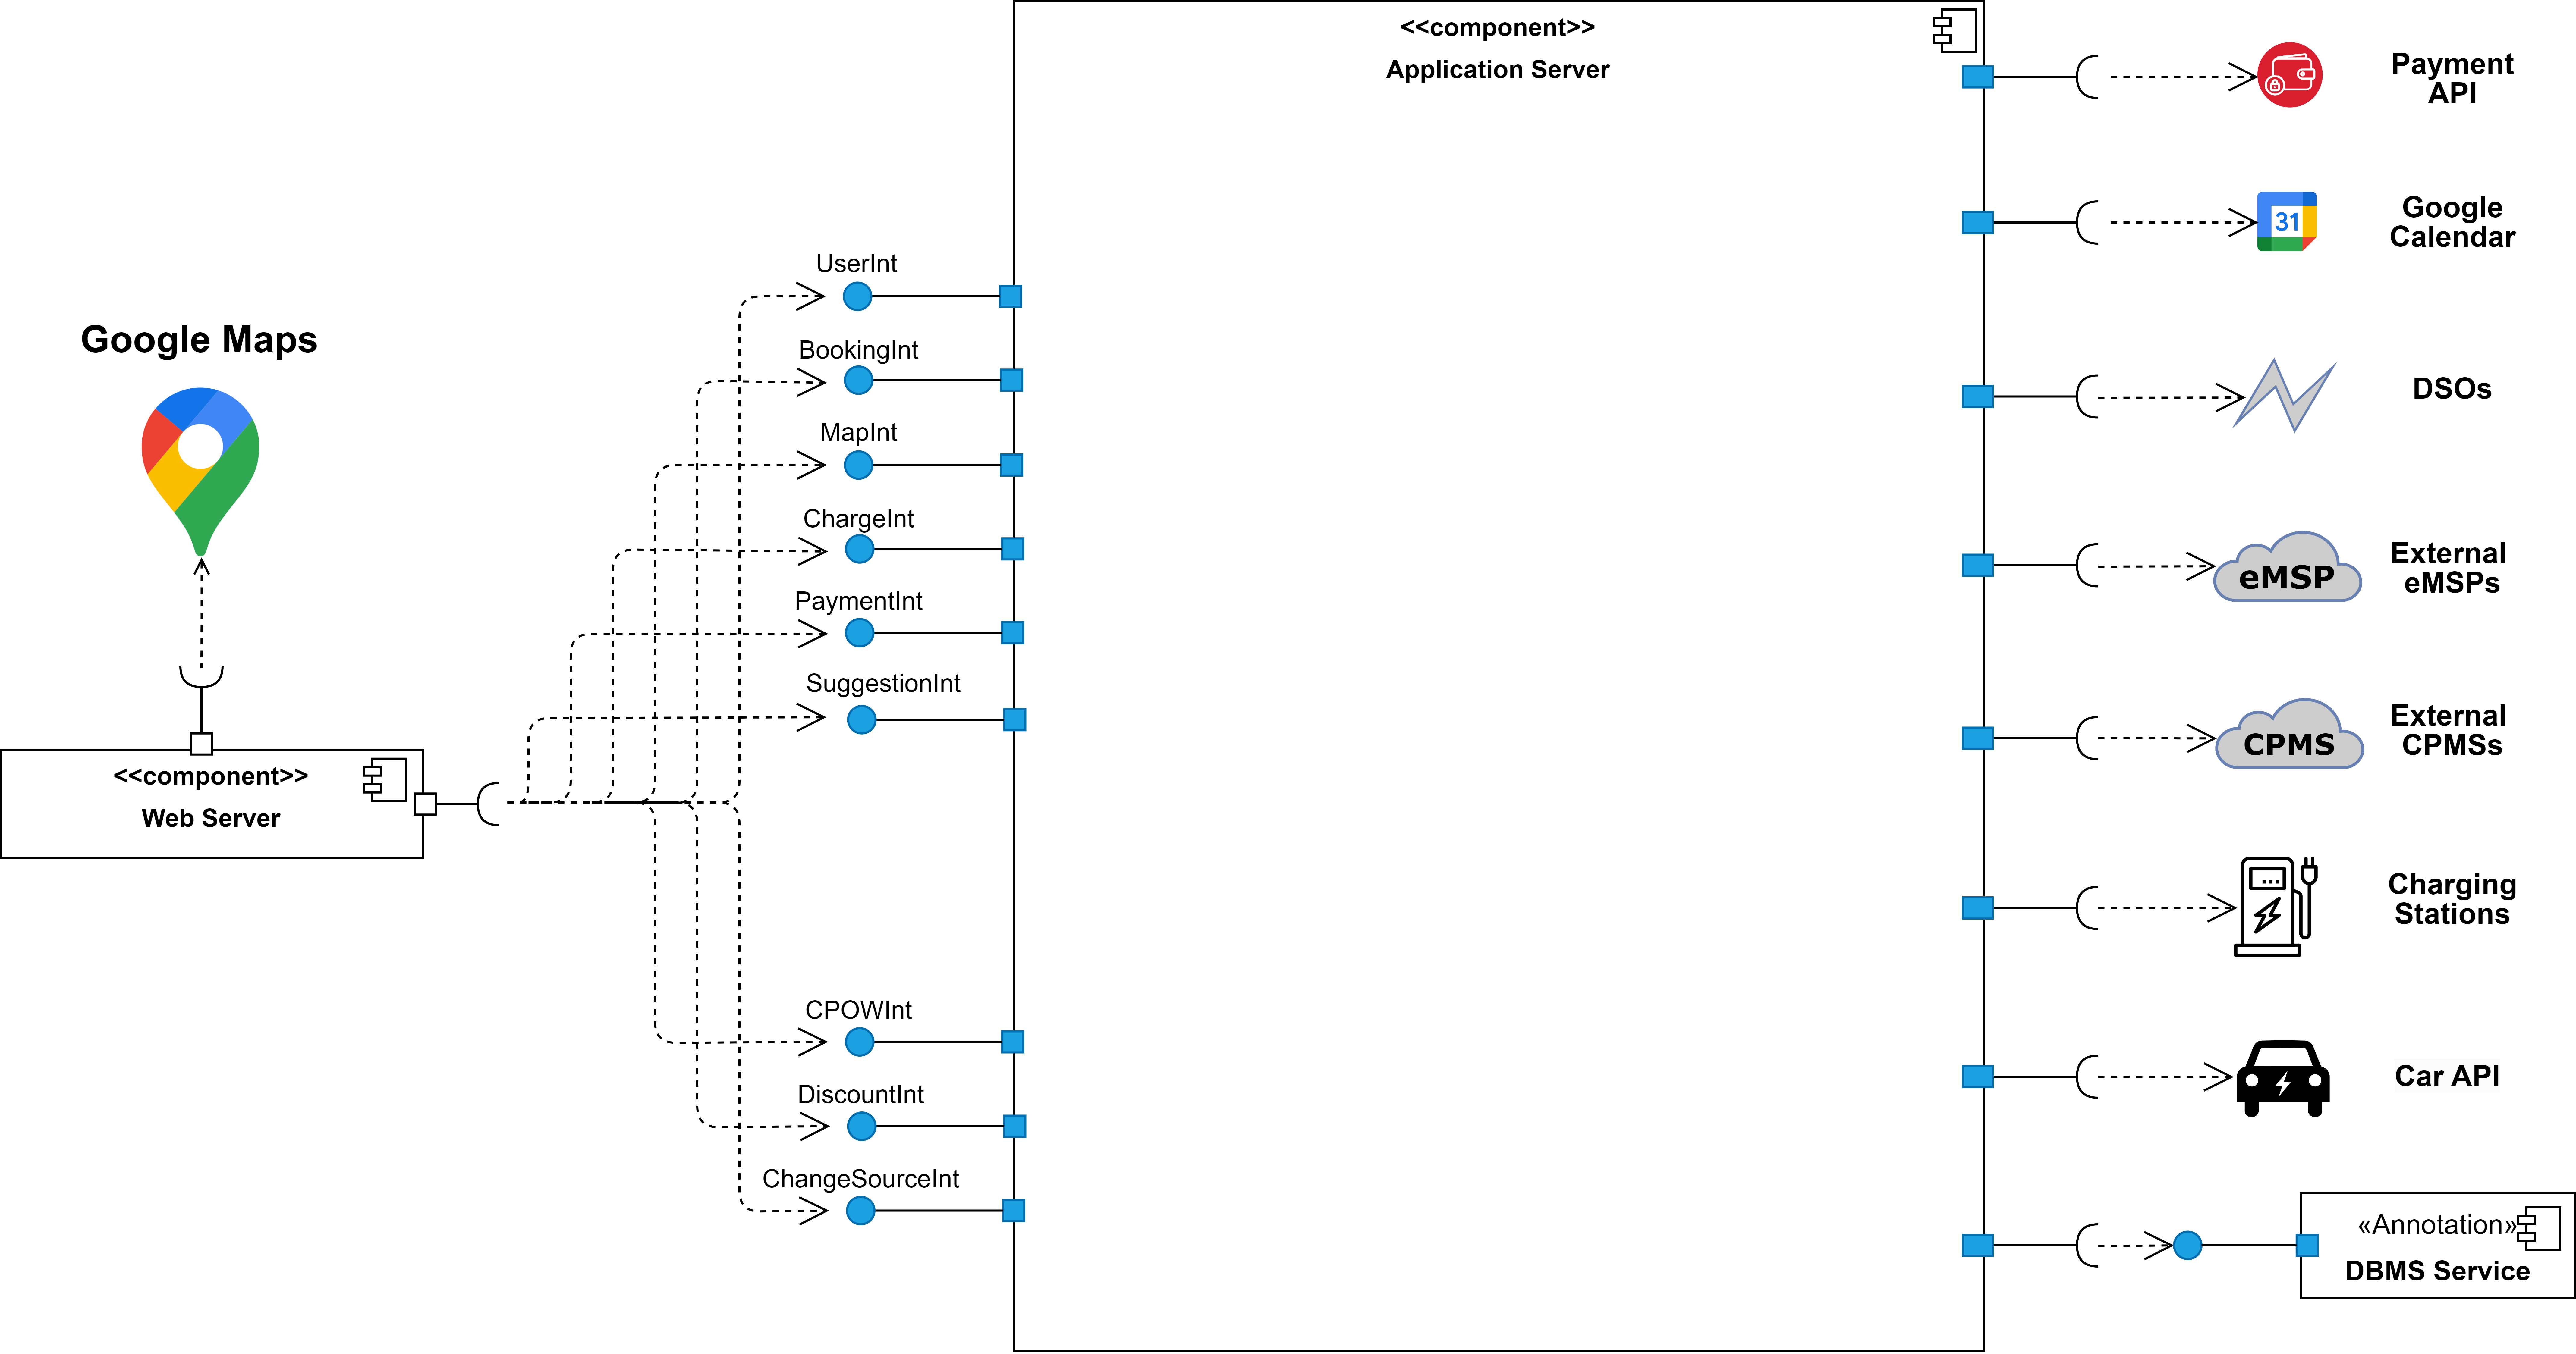
\includegraphics[scale=0.65, center]{assets/general_component_diagram.png}
        \caption{General Component Diagram}
        \label{fig: general_component_view}
    \end{figure}
\end{center}

This image gives a high level representation of the components of the system.
*description*

\subsubsection*{Application Server Component View}
\begin{center}
    \begin{figure}[H]
        \includegraphics[scale=0.33, center]{assets/application-server-component-diagram.png}
        \caption{Application Server Component Diagram}
        \label{fig: application_server_component_view}
    \end{figure}
\end{center}

The following component diagram gives a detailed view of the Application Server. It shows the internal structure and the interaction between the components.
External elements in the diagram are represented in a simplified way.

\begin{itemize}
    \item \textbf{first component}: description of compontent.
\end{itemize}

\subsubsection*{Web Server Component View}
Regarding the Web Server the main components are:
\begin{itemize}
    \item \textbf{first component}: description of component.
\end{itemize}

\newpage

\subsection{Deployment view}
\begin{center}
    \begin{figure}[H]
        
\includegraphics[scale=0.45, center]{assets/placeholder.png}
        \caption{Deployment Diagram}
        \label{fig: deployment_diagram}
    \end{figure}
\end{center}

The deployment diagram in \textit{Figure (\ref{fig: deployment_diagram})} shows the most important components necessary for the correct behaviour of the system.
The devices shown in the diagram are:
\begin{itemize}
    \item \textbf{first device/component}: description of device (e.g. pc or Smartphone, firewall, load balancer, web server, app server, database server...).
\end{itemize}
\newpage

\subsection{Runtime view}

Here the runtime views of some relevant use cases of the system are represented through sequence diagrams. 
In the diagrams, the part regarding the user is omitted because it has been deemed as redundant to the understanding of the interaction.
In later diagrams, some parts, like the login phase or returning to home page, were omitted for the the same motivations.

\newpage

\textbf{Sign Up}
\begin{center}
    \begin{figure}[H]
        
\includegraphics[scale=0.67, center]{assets/placeholder.png}
        \caption{Sign Up}
        \label{fig:signup}
    \end{figure}
\end{center}
*description of sign up as seen of the app by the user, with actions and final result*

\newpage

\textbf{Log In}
\begin{center}
    \begin{figure}[H]
        
\includegraphics[scale=0.8, center]{assets/placeholder.png}
        \caption{Log In}
        \label{fig: login}
    \end{figure}
\end{center}

The Log In phase simply consists in the user action of inserting their email (unique key in the database) and password in the login fields, then the system checks if the pair corresponds to a user entry in the database.
In case of success, the user can log in the system and use its functionalities available for that particular type of account chosen during the Sign Up phase.

\newpage

%the structure is the same for all these sections, just copy and paste

\textbf{*in app action 3*}
\begin{center}
    \begin{figure}[H]
        
\includegraphics[scale=0.70, center]{assets/placeholder.png}
        \caption{*in app action 3*}
        \label{fig: *in app action 3*}
    \end{figure}
\end{center}
description of the "app" action 3.

\newpage

%potrebbero esserci altre 6/7 sezioni come queste 3 sopra
%le immagini sono di sequence diagrams

\subsection{Component interfaces}

\begin{center}
    \begin{figure}[H]
        
\includegraphics[scale=0.60, center]{assets/placeholder.png}
        \caption{Component Interfaces Diagram}
        \label{fig: component_interfaces}
    \end{figure}
\end{center}

This diagram above describes in detail the interfaces and the corresponding methods offered by each component, it also shows the interaction between them.
*other text*

\subsection{Selected architectural styles and patterns}

    \begin{itemize}
        \item \textbf{type of architecture} \newline
             description and reasoning
        \item \textbf{Type of client} \newline
              description and reasoning
        \item \textbf{Scalability} \newline
              how can the architecture manage help scalability
        \item \textbf{MVC?} \newline
              general description
              \begin{itemize}
                  \item Model: the central component of the pattern. It is the application's dynamic data structure, independent of the user interface. It directly manages the data, logic and rules of the application.
                  \item View: The view defines how the app's data should be displayed.
                  \item Controller: it contains logic that updates the model and/or view in response to input from the users of the app. 
              \end{itemize}
    \end{itemize}

\newpage


\subsection{Other design decisions}
\label{other_design_decisions}
\subsubsection{Servers availability and response time} 
\label{server_availability}
text
\subsubsection{exaple of design decision} 
description of example

\begin{equation}
    possible\  equation \ to \ be \  included 
\end{equation}

development of said equation 

\begin{align}  
    description\ of\ development\ pt1\
    description\ of\ development\ pt2
\end{align}

other development and various considerations

%\begin{testexample}
%example of an application of our design decision (with data)
%\end{testexample}

 conclusion of design decision

 \subsubsection{design decision 2} 
    \begin{itemize}
        \item text
    \end{itemize}

\subsubsection{design decision 3} text

\newpage

\section{User Interface Design}
\begin{center}
    \begin{figure}[H]
        
\includegraphics[scale=0.74, center]{assets/placeholder.png}
        \caption{Sign Up and Log In}
        \label{fig: signMockup}
    \end{figure}
\end{center}

\begin{center}
    \begin{figure}[H]
        \vspace{-50px}
        
\includegraphics[scale=0.6, center]{assets/placeholder.png}
        \caption{carOwner interactions}
        \label{fig: agroMockup}
    \end{figure}
\end{center}

\begin{center}
    \begin{figure}[H]
        
\includegraphics[scale=0.6, center]{assets/placeholder.png}
        \caption{CPOW interactions}
        \label{fig: farmerInter}
    \end{figure}
\end{center}

\newpage

\section{Requirements Traceability}

\begin{longtable}{|p{0.47\textwidth}|p{0.45\textwidth}|}
    \hline
    \textbf{Requirements} & \textbf{Components} \\\hline\hline
    \begin{itemize}
        \item[R1)] text.
        \item[R2)] text.
        \item[R3)] text.
    \end{itemize}
    & 
    \begin{itemize}
        \item text.
        \item text.
        \item text.
    \end{itemize}
    \\\hline

    \begin{itemize}
        \item[R4)] text.
    \end{itemize}
    & 
    \begin{itemize}
        \item text.
    \end{itemize}
    \\\hline

    \begin{itemize}
        \item[R5)] text.
        \item[R6)] text.
        \item[R7)] text.
    \end{itemize}
    & 
    \begin{itemize}
        \item text.
        \begin{itemize}
            \setlength{\itemindent}{-5px}
            \item text.
            \item text.
            \item text.
        \end{itemize}
        \item text.
        \item text.
        \item text.
        \item text.
    \end{itemize}
    \\\hline

    \begin{itemize}
        \item[R8)] text.
    \end{itemize}
    & 
    \begin{itemize}
        \item text.
    \end{itemize}
    \\\hline

    \begin{itemize}
        \item[R9)] text.
    \end{itemize}
    &
    \begin{itemize}
        \item text.
        \begin{itemize}
            \item text.
        \end{itemize}
        \item text.
    \end{itemize}
    \\\hline

    \begin{itemize}
        \item[R10)] text.
    \end{itemize}
    &
    \begin{itemize}
        \item text.
        \begin{itemize}
            \item text.
        \end{itemize}
        \item text.
        \item text.
        \item text.
    \end{itemize}
    \\\hline

    \begin{itemize}
        \item[R11)] text.
    \end{itemize}
    &
    \begin{itemize}
        \item text.
        \begin{itemize}
            \item text.
        \end{itemize}
        \item text.
        \item text.
    \end{itemize}
    \\\hline

    \begin{itemize}
        \item[R12)] text.
    \end{itemize}
    &
    \begin{itemize}
        \item text.
        \begin{itemize}
            \item text.
        \end{itemize}
        \item text.
    \end{itemize}
    \\\hline

    \begin{itemize}
        \item[R13)] text.
        \item[R14)] text.
        \item[R15)] text. 
        \item[R16)] text.
        \item[R17)] text. 
    \end{itemize}

    &
    \begin{itemize}
        \item text. \begin{itemize}
            \item text.
        \end{itemize}
    \end{itemize}
    \\\hline

    \begin{itemize}
        \item[R18)] text.
    \end{itemize}
    &
    \begin{itemize}
        \item text. 
        \item text.
        \begin{itemize}
            \item text.
        \end{itemize}
    \end{itemize}
    \\\hline

    \begin{itemize}
        \item[R19)] text.
    \end{itemize}
    &
    \begin{itemize}
        \item text.
        \item text.
        \item text.
    \end{itemize}
    \\\hline

    \begin{itemize}
        \item[R20)] text. 
    \end{itemize}
    &
    \begin{itemize}
        \item text.
        \item text.
    \end{itemize}
    \\\hline
    \begin{itemize}
        \item[R21)] text.
    \end{itemize}
    &
    \begin{itemize}
        \item text.
    \end{itemize}\\\hline
\end{longtable}

Here, we present a summary of the table above for a more immediate visualization.
*component: name associated in the next table*
\begin{table}[H]
    \centering
    \begin{tabular}{|l l|}
        \hline
        component 1:& c1\\
        component 2:& c2\\\hline
        
    \end{tabular}
    \caption{Components' legend}
\end{table}
\newpage
\setlength\LTleft{-2.5cm}
\begin{longtable}{|c|c|c|}

    \hline
    & \cellcolor{blue!30}c1 & \cellcolor{blue!30}c2 \\\hline
    \cellcolor{SpringGreen!50}R1 & x & x \\\hline
    \cellcolor{SpringGreen!50}R2 & x & x \\\hline
    \cellcolor{SpringGreen!50}R3 & x & x \\\hline
    \cellcolor{SpringGreen!50}R4 & x &  \\\hline
    \cellcolor{SpringGreen!50}R5 &    & \\\hline
    \cellcolor{SpringGreen!50}R6 &    & \\\hline
    \cellcolor{SpringGreen!50}R7 &    & \\\hline
    \cellcolor{SpringGreen!50}R8 &    & \\\hline
    \cellcolor{SpringGreen!50}R9 &    & \\\hline
    \cellcolor{SpringGreen!50}R10 &    & \\\hline
    \cellcolor{SpringGreen!50}R11 &    & \\\hline
    \cellcolor{SpringGreen!50}R12 &    & \\\hline
    \cellcolor{SpringGreen!50}R13 &    & \\\hline
    \cellcolor{SpringGreen!50}R14 &    & \\\hline
    \cellcolor{SpringGreen!50}R15 &    & \\\hline
    \cellcolor{SpringGreen!50}R16 &    & \\\hline
    \cellcolor{SpringGreen!50}R17 &    & \\\hline
    \cellcolor{SpringGreen!50}R18 &    & \\\hline
    \cellcolor{SpringGreen!50}R19 &    & \\\hline
    \cellcolor{SpringGreen!50}R20 &    & \\\hline
    \cellcolor{SpringGreen!50}R21 & &\\\hline
    \caption{Component and requirement mapping}\\
\end{longtable}

\section{Implementation, Integration and Test Plan}
\subsection{Implementation Plan}
Multiple components will be implemented at the same time, in order to parallelize the development when possible. The general plan is to follow a bottom-up approach, so that core and basic functionalities with very few dependencies can be tested as soon as their incapsulating component is done. By doing so, the application will be built up with solid and tested foundations that will ease the further testing of bigger and complex components. In any case, unit testing will be performed on each component on the go, in order to find flaws out in advance. This will positevely impact the necessary actions to fix the faults since they will be done in an earlier stage.

The implementation's order of the component will be as follow:
\begin{enumerate}
    \item list, of, components
    \item list, of, components, 2
    \item list, of, components, 3
\end{enumerate}
Each group is composed by independent modules so they can be easily developed in parallel.
Furthermore, it is expected that external services (e.g. GoogleMapsAPI, *others* and DBMS Service) work properly since they're not a responsibility of the *name* app.

*explanation of the implementation plan component order*
\subsection{Integration Strategy}
Considering both the overall system's architecture and the implementation
plan, the chosen integration strategy is the bottom-up approach. System
integration begins with the integration of the lowest level modules and uses
test drivers to drive and pass appropriate data to the lower-level modules. As
and when the code for the other module gets ready, these drivers are replaced
with the actual module.

This approach allows to start the integration and testing without necessarily
waiting for the completion of the development and the unit testing of each
system's component. Being the low-level modules and their combined functions
often invoked by other modules, it is more useful to test them first so that
meaningful effective integration of other modules can be done. Moreover,
starting at the bottom of the hierarchy means that the critical modules are built
and tested first and therefore any errors in these modules are identified early in
the process.

Each integration in the same level (defined by the groups of the previous
section) is independent and there is no specific order in which to complete them.
In this way, the integration process and its testing are more flexible.

\subsubsection{Integration and Testing}
In this section it is defined the order of the integration between components. Test drivers will be used to simulate higher components not yet implemented.
*order of the components shown in the next figures, with references*

\begin{figure}[H]
    
\includegraphics[scale=0.6, center]{assets/placeholder.png}
    \caption{Integration of first component}
    \label{fig: integration_DataManager}
\end{figure}

\begin{figure}[H]
    \centering
    
\includegraphics[scale=0.6]{assets/placeholder.png} 
    \caption{Integration of second component}%
    \label{fig: integration_MapServiceManager_WeatherManager}%
\end{figure}

\begin{figure}[H]
    \centering
    \subfloat[\centering component 3a]{{
\includegraphics[scale=0.5]{assets/placeholder.png}}}%
    \qquad\qquad
    \subfloat[\centering component 3b]{{
\includegraphics[scale=0.5]{assets/placeholder.png}}}%
    \caption{Integration of 3a and 3b components}%
    \label{fig: integration_SensorDataManager_NewsManager}%
\end{figure}

*order of components for the middle tier, with references*
\begin{figure}[H]
    \centering
    \subfloat[\centering component middle1-a]{{
\includegraphics[scale=0.5]{assets/placeholder.png}}}%
    \qquad\qquad
    \subfloat[\centering component middle1-b]{{
\includegraphics[scale=0.5]{assets/placeholder.png}}}%
    \qquad\qquad
    \subfloat[\centering component middle1-c]{{
\includegraphics[scale=0.7]{assets/placeholder.png}}}%
    \caption{Integration of middle1-a,b,c components}%
    \label{fig: integration_RankingManager_HelpRequestManager}%
\end{figure}
\begin{figure}[H]
    \centering
    
\includegraphics[scale=0.55]{assets/placeholder.png}%
    \caption{Integration of middle2 component}%
    \label{fig: integration_ForumManager_LocationModule}%
\end{figure}

*order of last group components, with references to the images*

\begin{figure}[H]
    \centering
    
\includegraphics[scale=0.6, center]{assets/placeholder.png}
    \caption{Integration of carOwnerManager components}
    \label{fig: integration_PolicyMakerManager}
\end{figure}
\begin{figure}[H]
    \centering
    
\includegraphics[scale=0.6, center]{assets/placeholder.png}
    \caption{Integration CPOWmanager components}
    \label{fig: integration_AgronomistManager}
\end{figure}
\begin{figure}[H]
    \centering
    
\includegraphics[scale=0.6, center]{assets/placeholder.png}
    \caption{Integration of otherManager components}
    \label{fig: integration_FarmerManager}
\end{figure}
\begin{figure}[H]
    \centering
    
\includegraphics[scale=0.7, center]{assets/placeholder.png}
    \caption{Integration of AccountManager components}
    \label{fig: integration_AccountManager}
\end{figure}

\subsection{System testing}
*text for sys testing*
\newpage
\section{Effort Spent}
    \begin{tabular}{|c||c|c|c|c|c|}
        \hline
        Student & Time for S.1 & S.2 & S.3 & S.4 & S.5\\ \hline
        stud1 & 0h & 0h & 0h & 0h & 0h \\
        stud2 & 0h & 0h & 0h & 0h & 0h \\
        stud3 & 0h & 0h & 0h & 0h & 0h \\
        \hline
    \end{tabular}


\section{References}


\begin{thebibliography}{9}
    \bibitem{reference1}
    MDN Web Docs Glossary: Definitions of Web-related terms -> MVC
    \url{https://developer.mozilla.org/en-US/docs/Glossary/MVC}

    \bibitem{reference2}
    description: \url{url here}
    
\end{thebibliography}

\end{document}